\chapter{Indledning}
Hensigten med dette projekt er at udvikle spillet \textit{Goofy Candygun 3000}. Spillet går ud på, at 1-2 spillere dyster om at ramme et mål med slik affyret fra en slikkanon styret af en Wii-Nunchuck controller. For at finde inspiration til projektet og idéer til implementering blev der søgt efter lignende projekter på internettet. Det viste sig, at idéen med at skyde med slik, ikke er en original idé, da lignende projekter såsom \textit{The Candy Cannon} \cite{CandyCannon} allerede findes. Til forskel fra The Candy Cannon og lignende projekter som affyrer projektiler uden et egentlig formål, vil der i dette projekt blive udviklet en kanon til brug i et spil. 
Målet med projektet, er at bygge en funktionelt prototype, samt at dokumentere dette med en projektrapport og dens dertilhørende dokumentationdokument. 
Det følgende afsnit beskriver, hvilke krav der stilles til projektet fra IHA's side.

\section{Krav til produktet}
Projektet tager udgangspunkt i projektoplægget for 3. Semesterprojektet, præsenteret af \textit{Ingeniørhøjskolen, Aarhus Universitet} (Bilag/Projektrapport/Semesterprojekt3Oplæg). Til dette projekt er der ikke stillet krav til typen af produkt der skal udvikles, dog er der sat krav til hvad produktet skal indeholde. Disse krav er som følger:

\begin{itemize}
	\item{Systemet \textit{skal} via sensorer/aktuatorer interagere med omverdenen}
	\item{Systemet \textit{skal} have en brugergrænseflade}
	\item{Systemet \textit{skal} indeholde faglige elementer fra semesterets andre fag}
	\item{Systemet \textit{skal} anvende en indlejret Linux platform og en PSoC platform}
\end{itemize}

\noindent I dette projekt bliver produktet opbygget som en prototype. Grundet dette er der i afsnit \ref{afsnit:analyse} beskrevet, og begrundet for, nogle grundlæggende hardwarekomponenter til realisering af denne prototype.


\section{Systembeskrivelse}
\label{afsnit:systembeskrivelse}
I dette projekt skal der udvikles en slik kanon, som skal bruges i et nyt spil som kommer til at hedde \textit{Goofy Candygun 3000}. Denne slik kanon skal kunne skyde med slik. Kanonen, der affyrer slikket, skal styres af spillerne via en Wii-Nunchuck controller. Spillet vil have en brugergrænseflade, hvor brugeren kan vælge spiltype, og se statistikker og point for hvert spil. \newline

\noindent Et typisk brugerscenarie er, at spillerne bestemmer antallet af skud for runden. Når dette er gjort, er spillet igang. Herefter går Wii-nunchucken på skift mellem spillerne for hvert skud. Dette fortsættes indtil skuddene er opbrugt. Vinderen er spilleren med flest point. Spillets statistikker vises løbende på brugergrænsefladen. Dette brugerscenarie er illustreret i det rige billede på figur \ref{fig:RigtBillede}.

\begin{figure}[H]
	\centering
	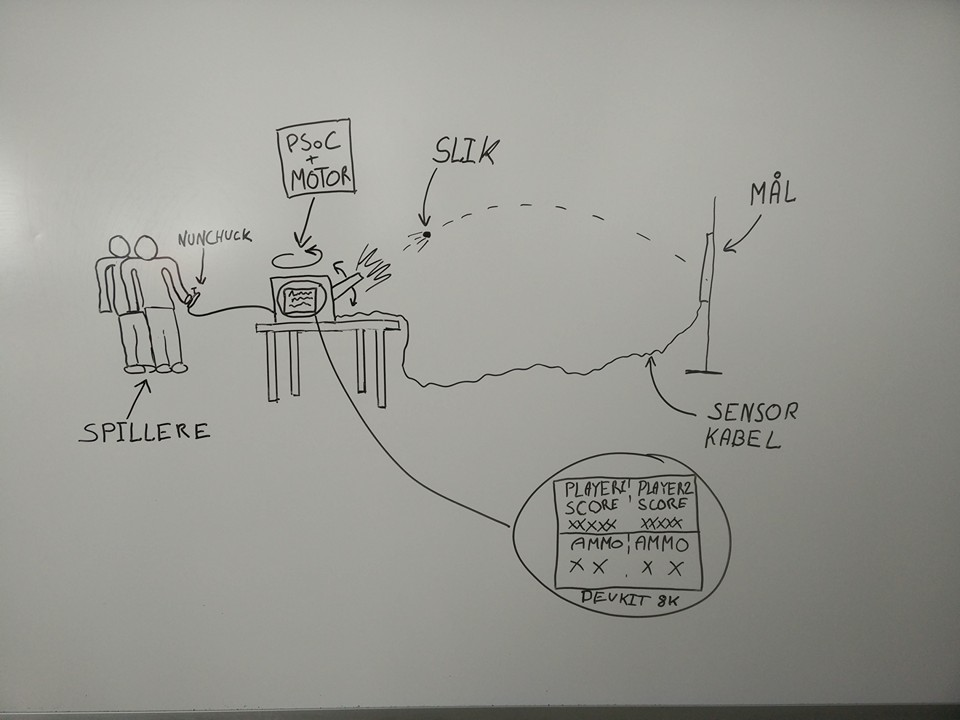
\includegraphics[width=\textwidth]{Projektformulering/images/rigtBillede}
	\caption{Illustration af brugsscenarie for Goofy Candygun 3000}
	\label{fig:RigtBillede}
\end{figure}

Det endelige produkt, hvis alle ønsker til produktet opfyldes, omfatter:
\begin{itemize}
	\item{En brugergrænseflade, hvor brugeren kan initiere både system test og selve spillet. Derudover kan brugergrænsefladen vise:}
	\subitem{Point}
	\subitem{Kanonens vinkel}
	\subitem{Antal resterende skud}
	\item{Består af 3 motorer, der drejer kanonen om forskellige akser}
	\subitem{Disse skal styres med en Wii-nunchuck controller}
	\subitem{To af motorerne styrer kanonen i forskellige retninger, og den sidste er til at affyre kanonen}
	\item{Et mål, der kan registrere spillernes skud}
	\item {Muligheden for at flere spillere kan spille sammen}
\end{itemize}

\noindent Brugergrænsefladen vil blive implementeret på et Devkit 8000. Denne vil kommunikere med et netværk af PSoC udviklingsboards, der tager input fra en Wii-Nunchuck, og fortolker disse til signaler, for at styre kanonens motorer.
